\chapter{Results and Discussion}

Based on the preceding analysis, following parameters were derived for each vessel, assuming they will engage in similar trade flows as observed in 2022, but in the year 2023. 
The vessels have been categorized into segments, facilitating a more intricate examination of the outcomes. The segments encompassed within this report include Capesize, Panamax, Supramax, Aframax, Suezmax, VLGC, and VLCC.

The analysis encompassed a total of 9,406 vessels. 
The parameters acquired for each vessel comprise an array of emissions and indices, contributing to a comprehensive assessment. 
These parameters encompass CO2 emissions, SO2 emissions, NOx emissions, PM emissions, NMVOC, CH4, N2O, CO, Black Carbon, Organic Carbon, EEOI, CII, and CII grade.

\section{Grade Distribution}

\begin{figure}[h]
    \centering
    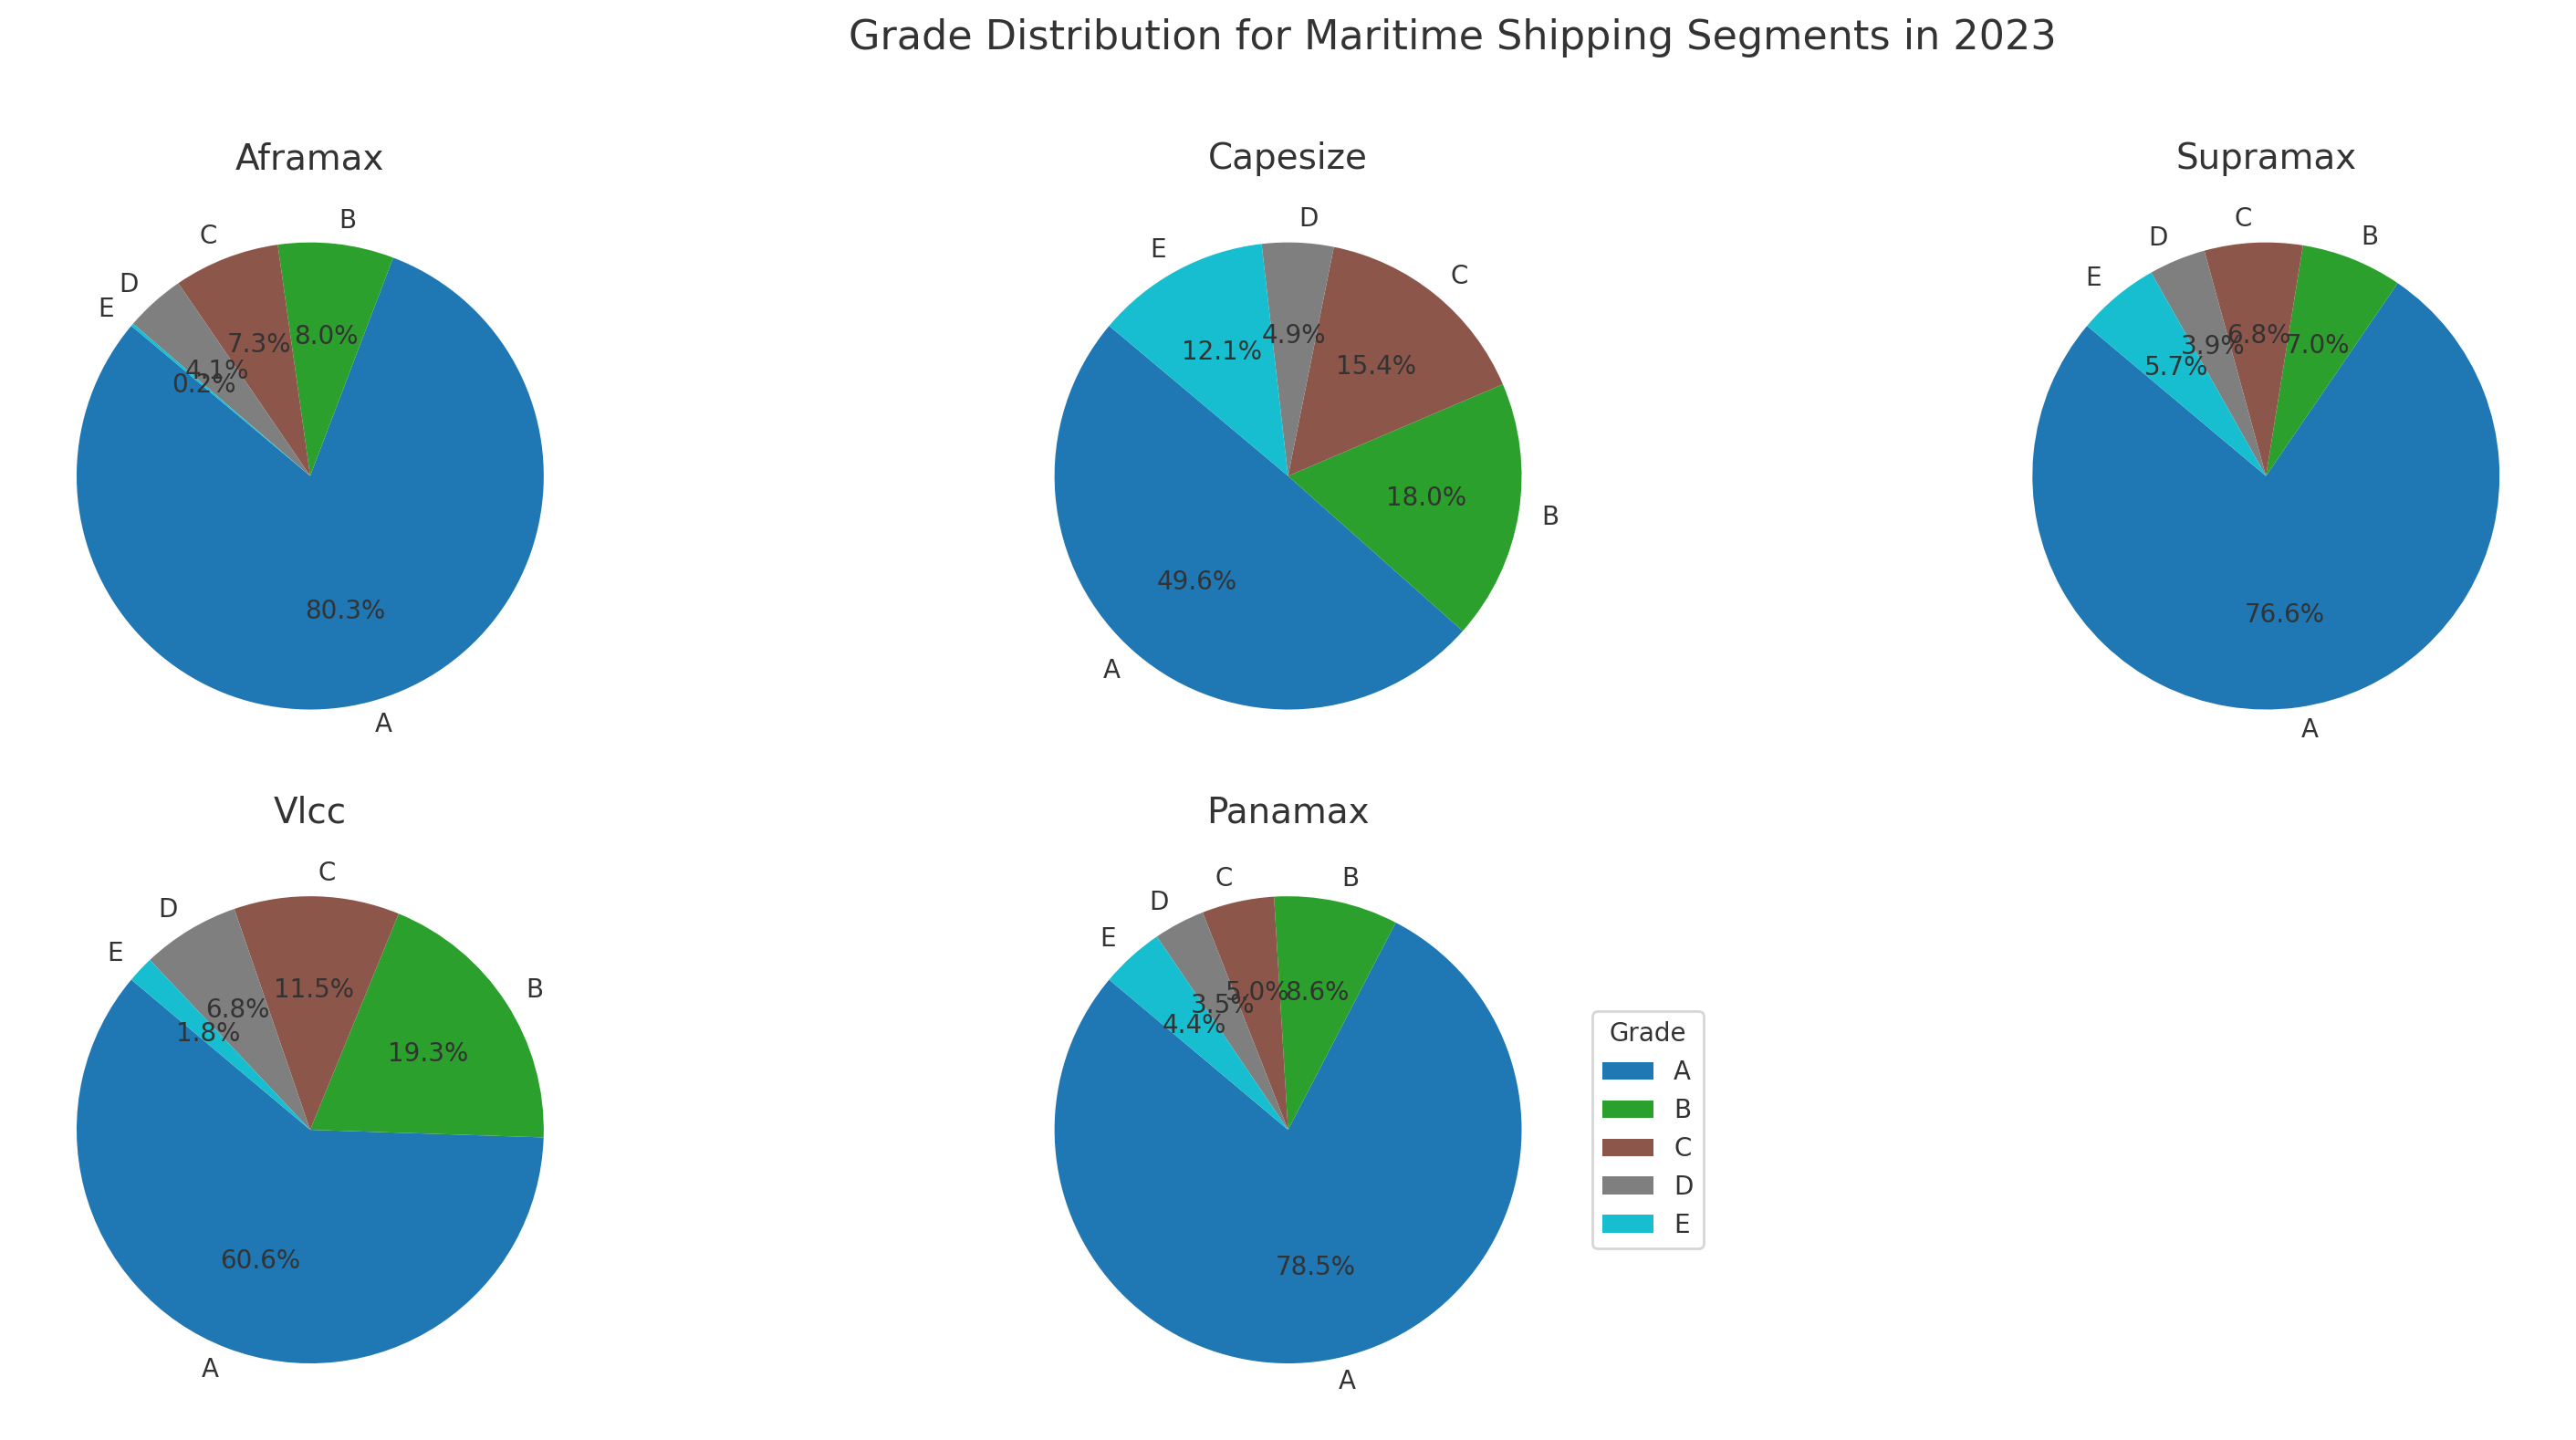
\includegraphics[width=0.8\textwidth]{images/grade_distribution.png}
    \caption{Grade Distribution}
    \label{grade_distribution}
\end{figure}


\begin{figure}[h]
    \centering
    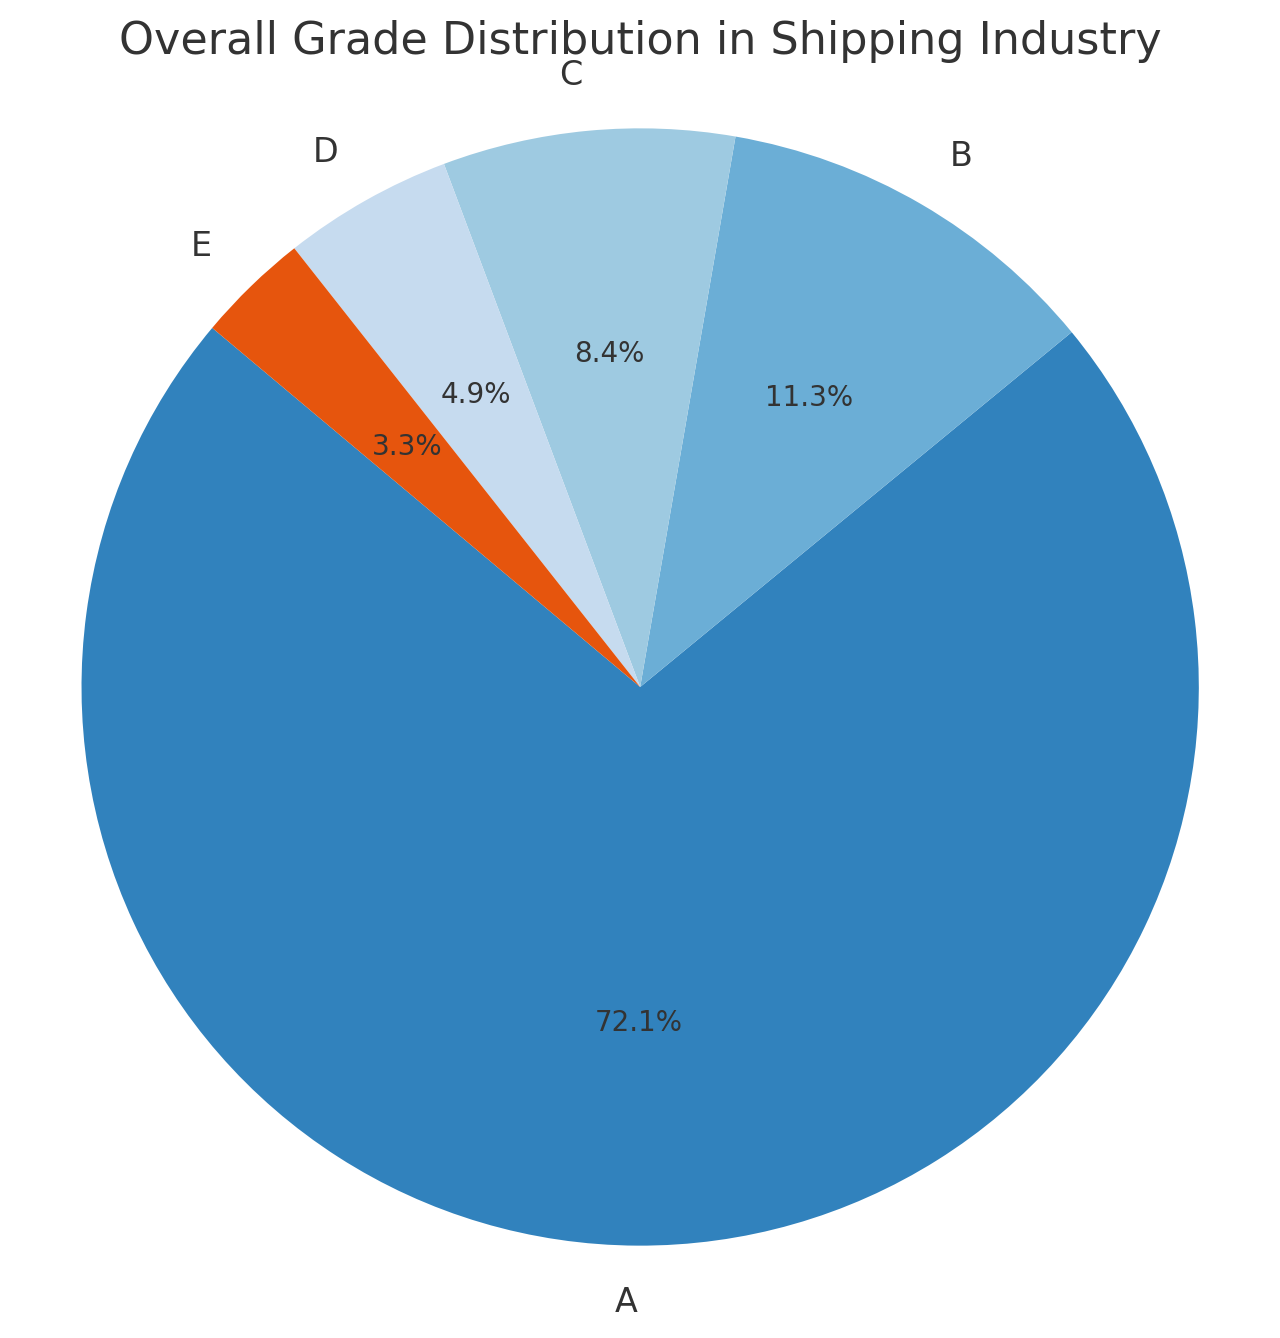
\includegraphics[width=0.8\textwidth]{images/combined_grade.png}
    \caption{Combined Grade}
    \label{combined_grade}
\end{figure}

The pie chart analysis of vessel grades across different maritime shipping segments in Figure \ref{grade_distribution}, 
along with the combined view in Figure \ref{combined_grade}, offers a nuanced understanding of the quality and compliance distribution within the industry as of 2023.


Most of segments shows similar distribution of grades, with Grade A being in between 60\% to 80\% while Grade D and E being around 10\%.
This can be reflected in combined chart too. Though capesize is an exception with only about 50\% of vessels in Grade A and alomst 16\% with grade D and E.

The combined pie chart encapsulates the overall landscape, showing 69.5\% of vessels in Grade A, and 10\% in Grade D and E.

The segment-specific insights reveal subtle variations that may be influenced by factors such as vessel size, purpose, technological capabilities, and market demands. 
Understanding these variations is essential for targeted interventions and strategies to further enhance quality and compliance.

In conclusion, the pie chart analysis paints a vivid picture of the maritime shipping industry's commitment to high standards as reflected in the grades. 
It also emphasizes the need for continuous innovation, particularly in the face of stricter grading systems in the future. 
The segment-wise insights provide valuable guidance for industry stakeholders, regulators, and policymakers, facilitating data-driven decision-making and fostering a culture of continuous improvement and adaptation.


\section{Projected Grade Trend}

\begin{figure}[h]
    \centering
    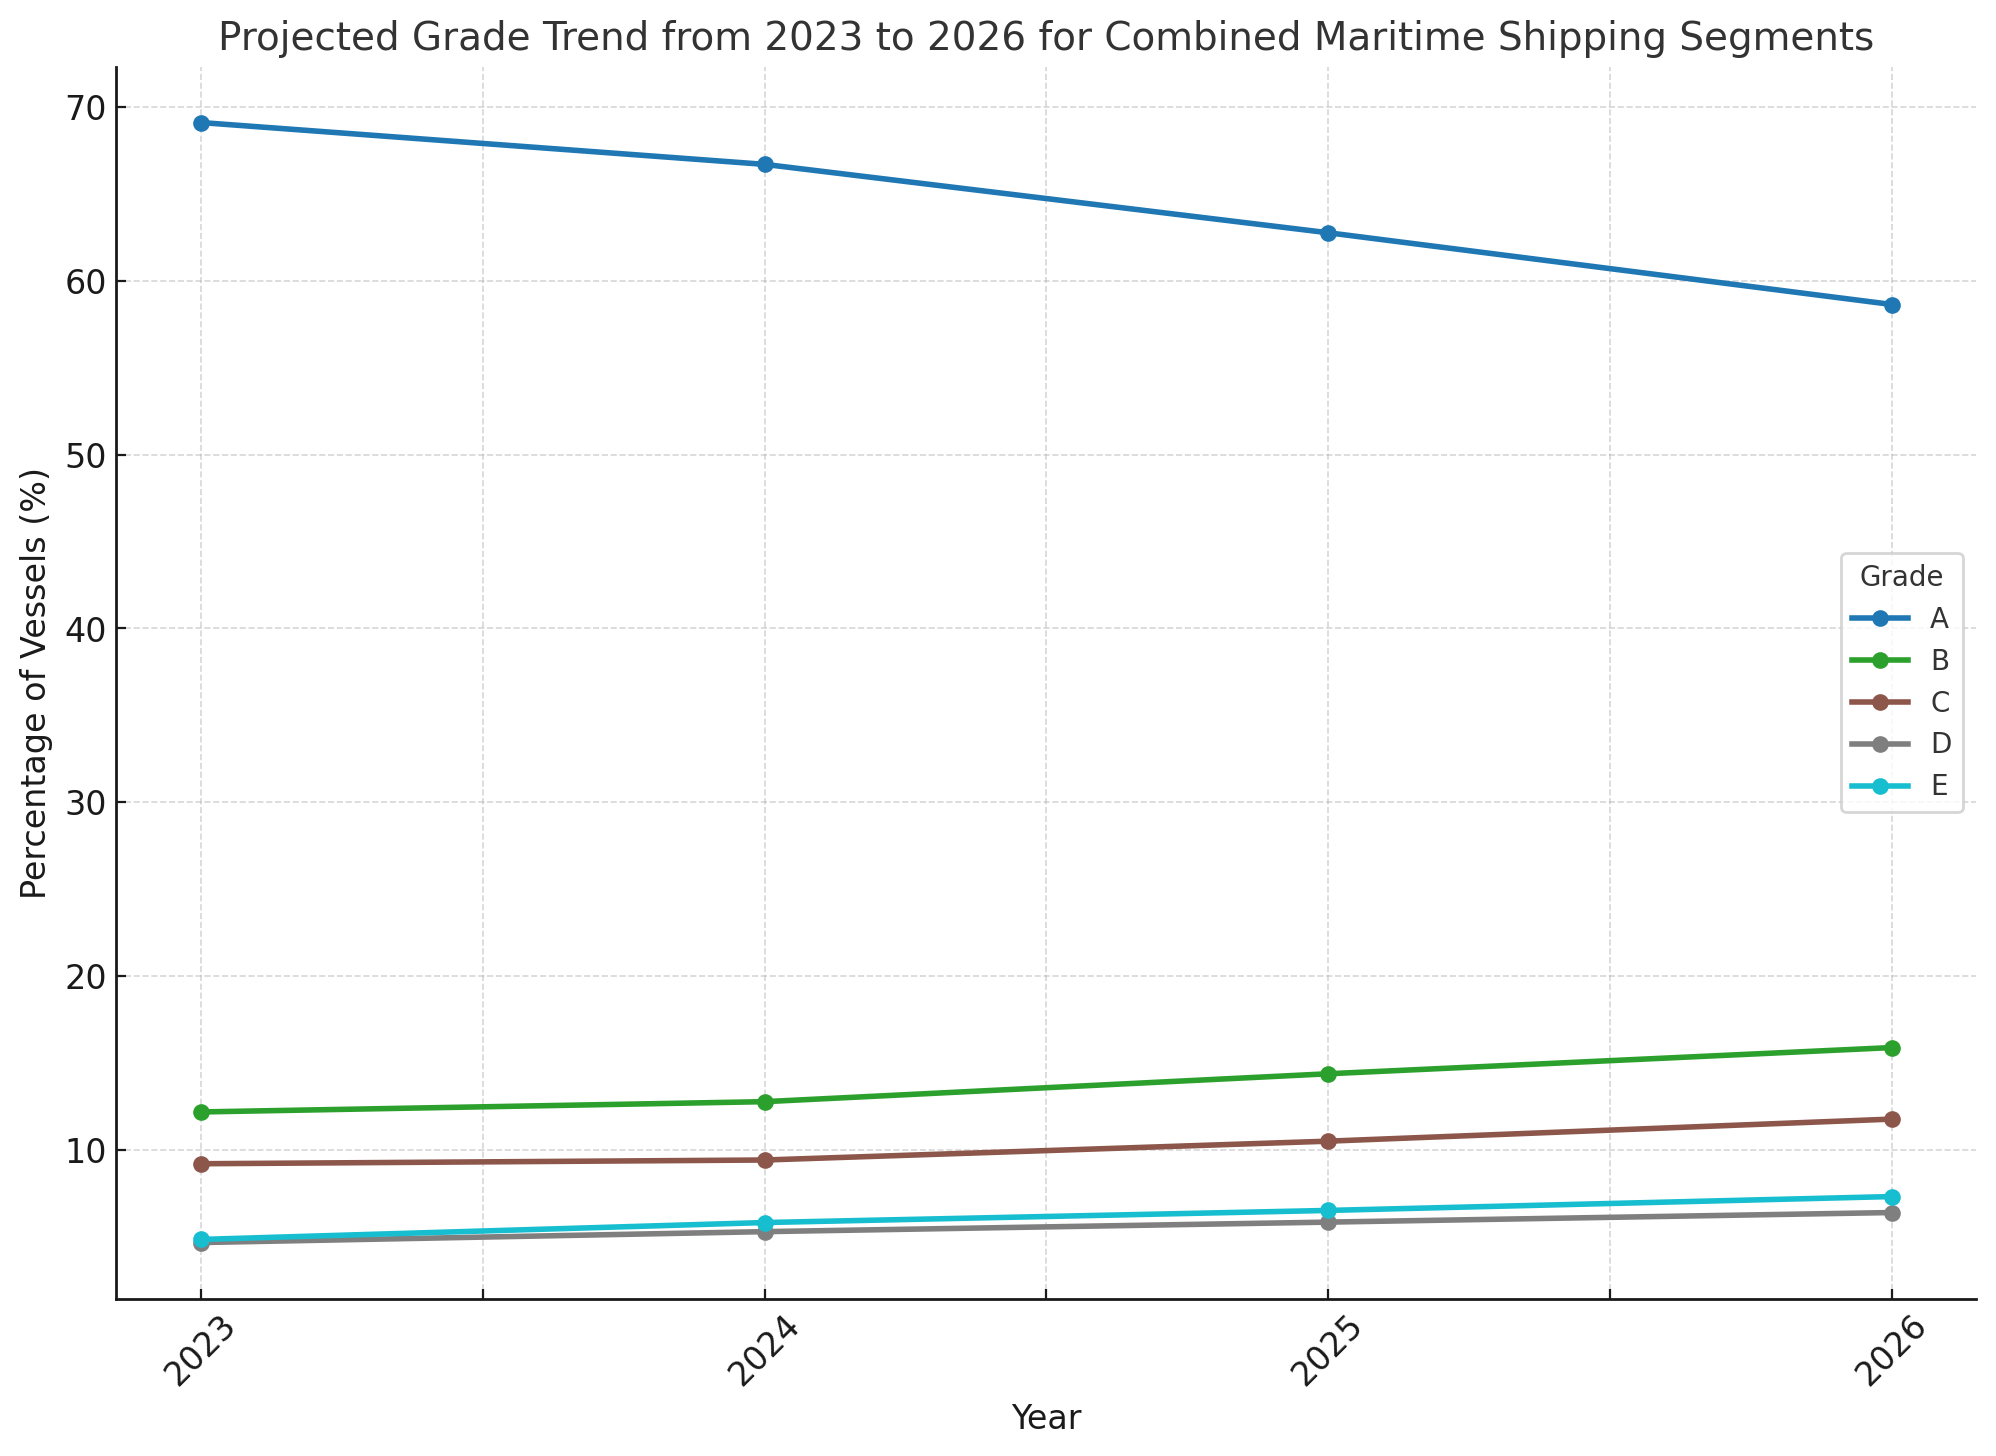
\includegraphics[width=0.8\textwidth]{images/grade_trend.png}
    \caption{Projected Grade Trend}
    \label{grade_trend}
\end{figure}

The analysis of the projected grade trend from 2023 to 2026 in plot \ref{grade_trend} unveils a compelling narrative of the industry's response to an increasingly stringent grading system. 
The most pronounced observation is the decline in the percentage of vessels achieving Grade A, falling from 69\% in 2023 to less than 60\% in 2026. 
This reduction is not indicative of a decline in quality or compliance but rather a reflection of the escalating standards and criteria set by the grading authorities.

This trend underscores the industry's challenge to keep pace with evolving regulations and the imperative for continuous innovation and improvement. 
As the grading system becomes more demanding, the criteria for achieving Grade A are elevated, pushing some vessels into the B and C categories. 
The growth in Grades B and C, from about 12.18\% to 16\% and 9\% to 12\% respectively, illustrates this shift.

Even the slight increases in Grades D and E, though representing a smaller fraction of the fleet, emphasize the pressing need for maritime shipping to adapt, innovate, and invest in new technologies and practices. 
The trend towards more rigorous grading is likely driven by global efforts to enhance environmental sustainability, safety standards, and overall efficiency within the maritime sector.

The observed grade trend serves as both a challenge and an opportunity for maritime shipping. 
It calls for a proactive and strategic approach, where shipping companies must embrace research and development, adopt advanced technologies, and foster a culture of excellence. 
The industry must recognize that the path to high grades is dynamic and requires ongoing commitment to align with the progressive standards.

In conclusion, the projected grade trend from 2023 to 2026 is a testament to the maritime shipping industry's evolving landscape. 
It emphasizes the critical role of innovation in meeting the future demands of a stricter grading system. 
This trend offers valuable insights for policymakers, regulators, and industry leaders, guiding them towards collaborative efforts that ensure the maritime shipping industry not only maintains its current standards but continually strives to reach new heights of quality and responsibility.

\section{EEOI vs Grade}

\begin{figure}[h]
    \centering
    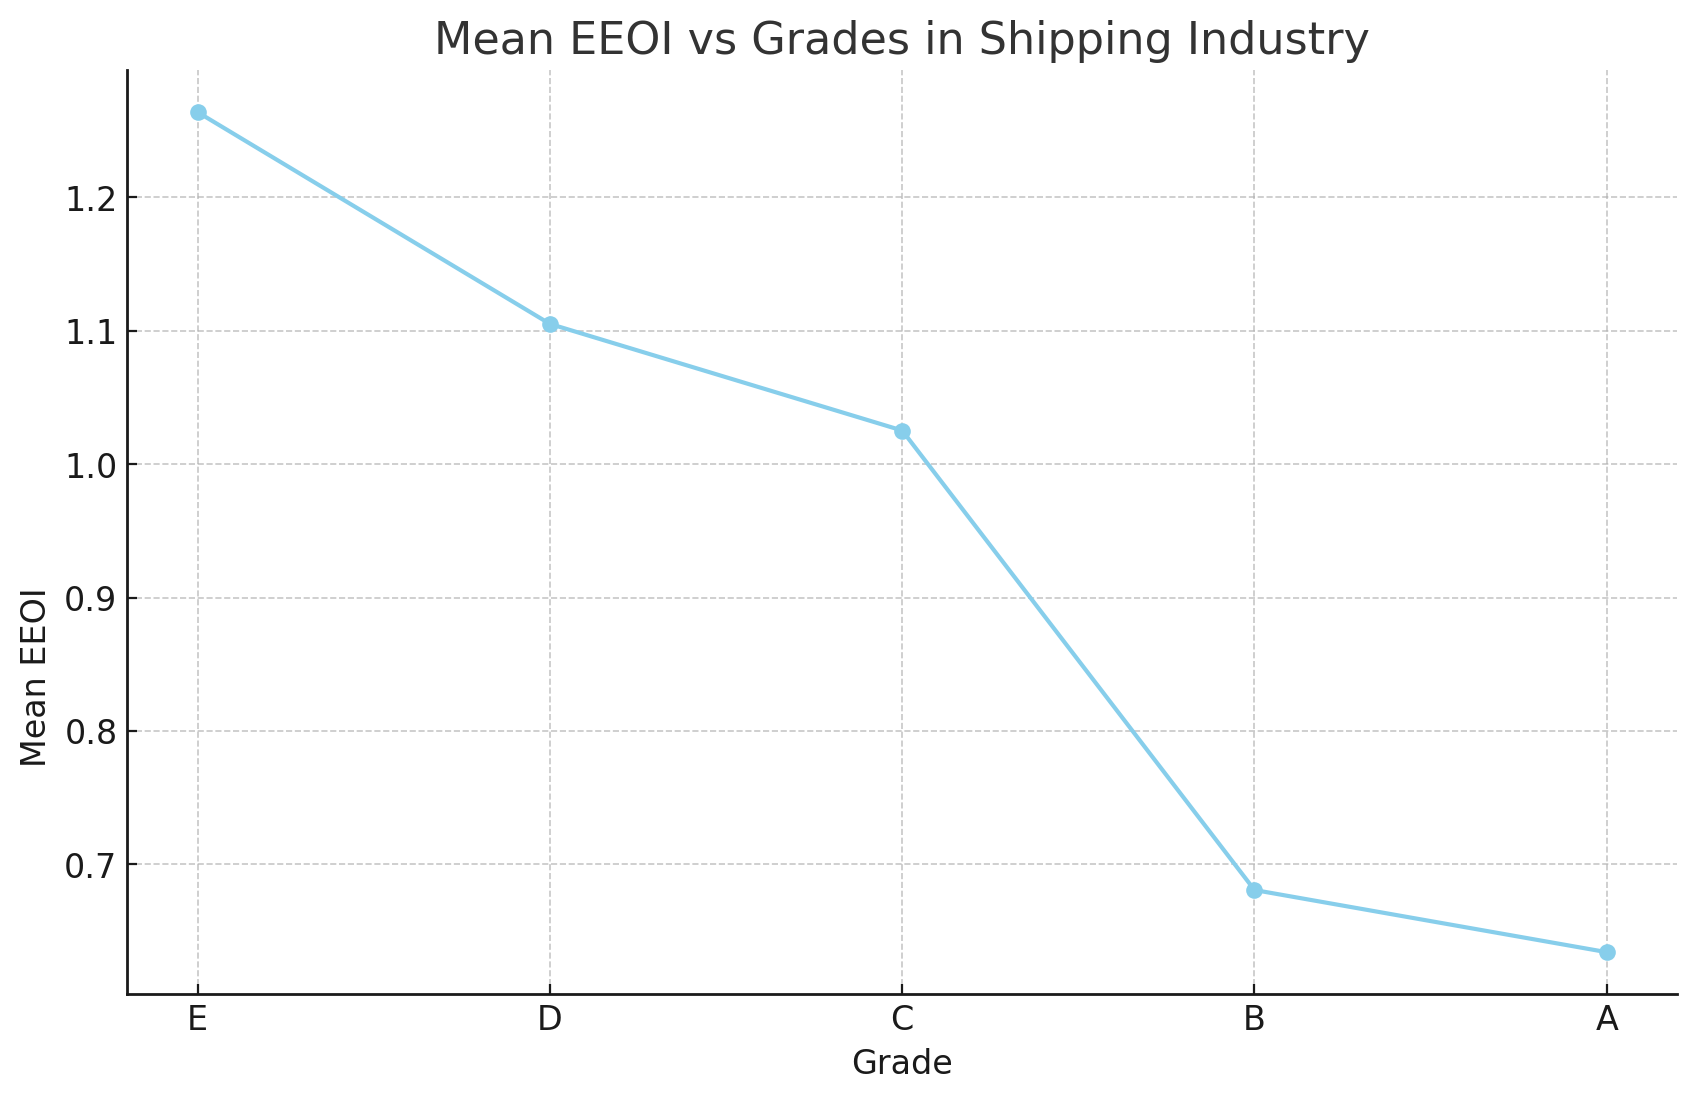
\includegraphics[width=0.8\textwidth]{images/eeoi_grade.png}
    \caption{Mean EEOI vs Grade}
    \label{eeoi_grade}
\end{figure}

The above Figure \ref{eeoi_grade} represnts realtionship between EEOI and grade.

Lower Efficiency Operational Indicator (EEOI) means vessels uses less fuel to achive same amount of work.
The relationship between the Energy EEOI and vessel grades in the maritime shipping industry offers a logical and meaningful correlation. 
Lower EEOI values, signifying better energy efficiency, correspond to higher vessel grades (A being the highest). 
The grading system incentivizes energy-efficient practices and provides a transparent metric for evaluating vessel quality and environmental responsibility.

\section{Average speed vs Grade}
\begin{figure}[h]
    \centering
    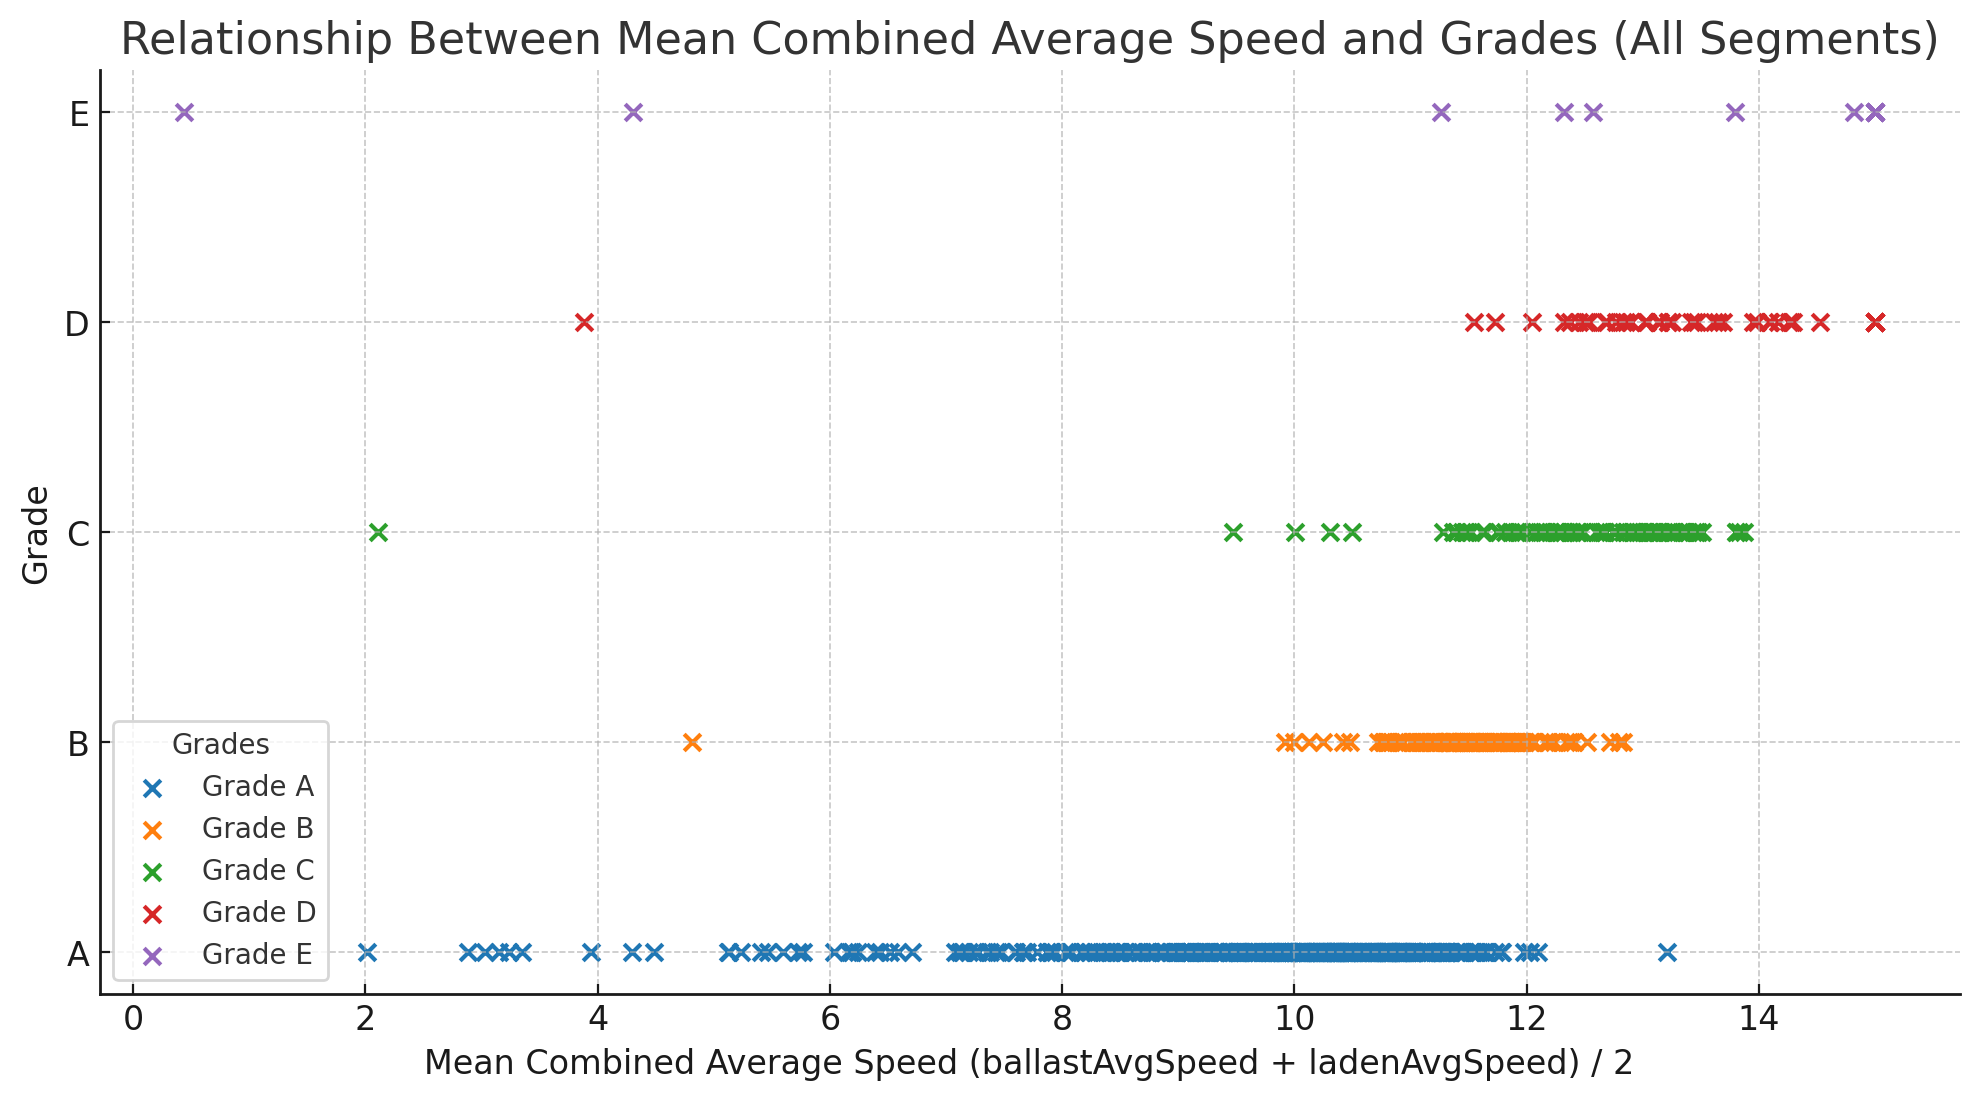
\includegraphics[width=0.8\textwidth]{images/grade_speed.png}
    \caption{Average Speed vs Grade}
    \label{grade_speed}
\end{figure}

To understand if speed has any impact on grade, scatter plot of average speed vs grade is plotted.
From the plot \ref{grade_speed} it is noticed that vessels with lower speed have better grade. 
It is very clear that almost all the vessels with speed 12.5 knots or more have grade C or below.

\section{Grade by Build Country}

\begin{figure}[h]
    \centering
    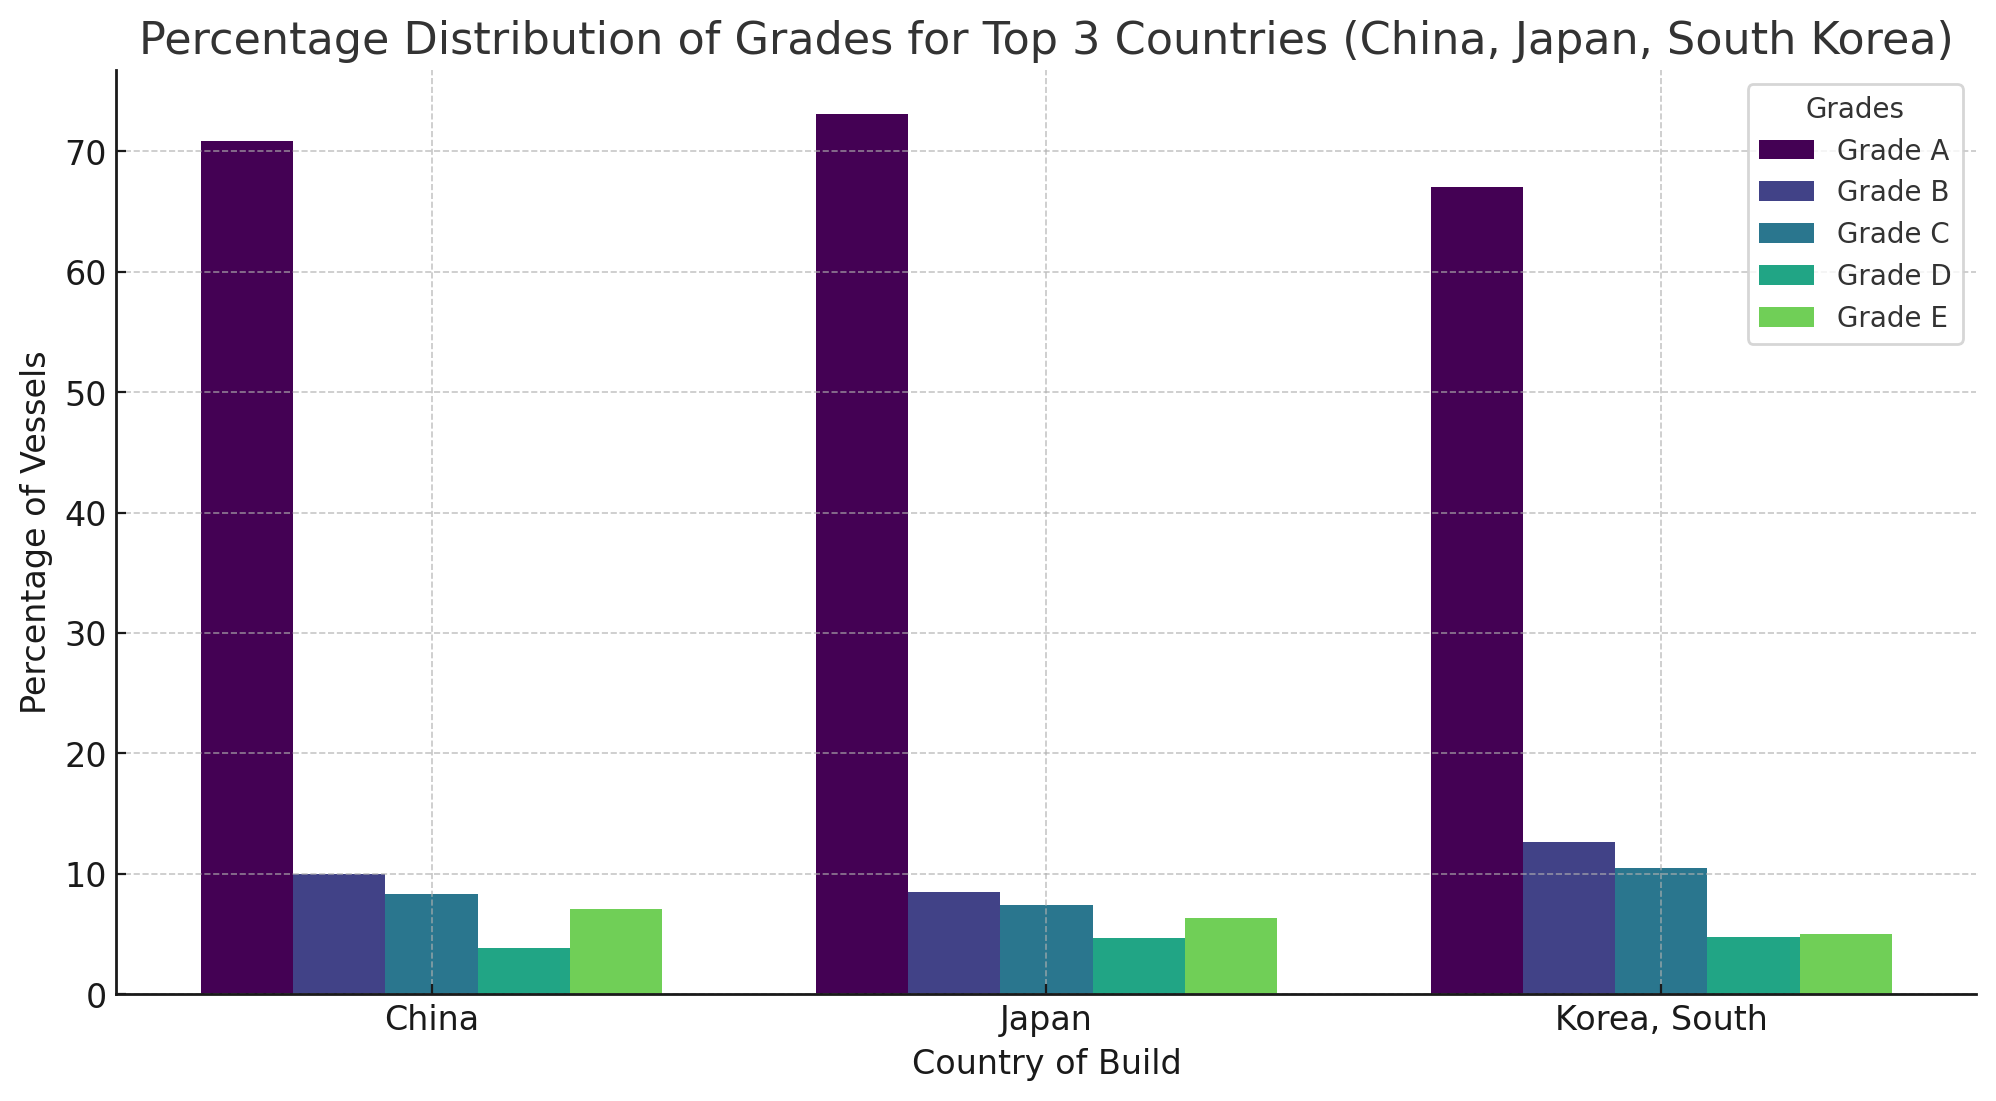
\includegraphics[width=0.8\textwidth]{images/grade_by_build_country.png}
    \caption{Grade By Build Country}
    \label{grade_by_build_country}
\end{figure}

Country where vessels are built can effect grade significantly as many parameters like materials, technology, regulations etc. can vary from country to country.
To verify this hypothesis, grade distribution by build country is plotted in Figure \ref{grade_by_build_country}.
To make the plot more readable, only top 3 countries China, Japan and South Korea were considered.

From plot \ref{grade_by_build_country} it is clear that vessels built in Japan have better grade than vessels built in China or South Korea.

\section{Addressing Low Rating}

When a ship's Carbon Intensity Indicator (CII) receives a low grade of D for three consecutive years or E for one year, specific measures must be undertaken to address and improve the situation. 
As per the regulations, a corrective action plan must be submitted and approved. 

Some of the strategies include the use of alternative fuels, which may require significant investment but have high effectiveness; 
the application of low friction paint and Energy Saving Devices (ESD) to improve hardware; 
voyage optimization and fleet optimization, which may require preliminary examination but have a low to middle cost and depend on the ship's specific situation; 
and slow steaming, which requires an analysis of monitoring results and estimation of cost-effectiveness. 
These methods indicate a multifaceted approach that considers cost, effectiveness, and specific ship characteristics to overcome the challenges associated with a low CII rating. 
The strategies emphasize both technological improvements and operational adjustments, reflecting an integrated approach to enhance environmental performance.


\section{Emissions}

Based on AF code emission API and vessel parameters, various emissions are calculated for each vessel grouped by segment.

\begin{figure}[h]
    \centering
    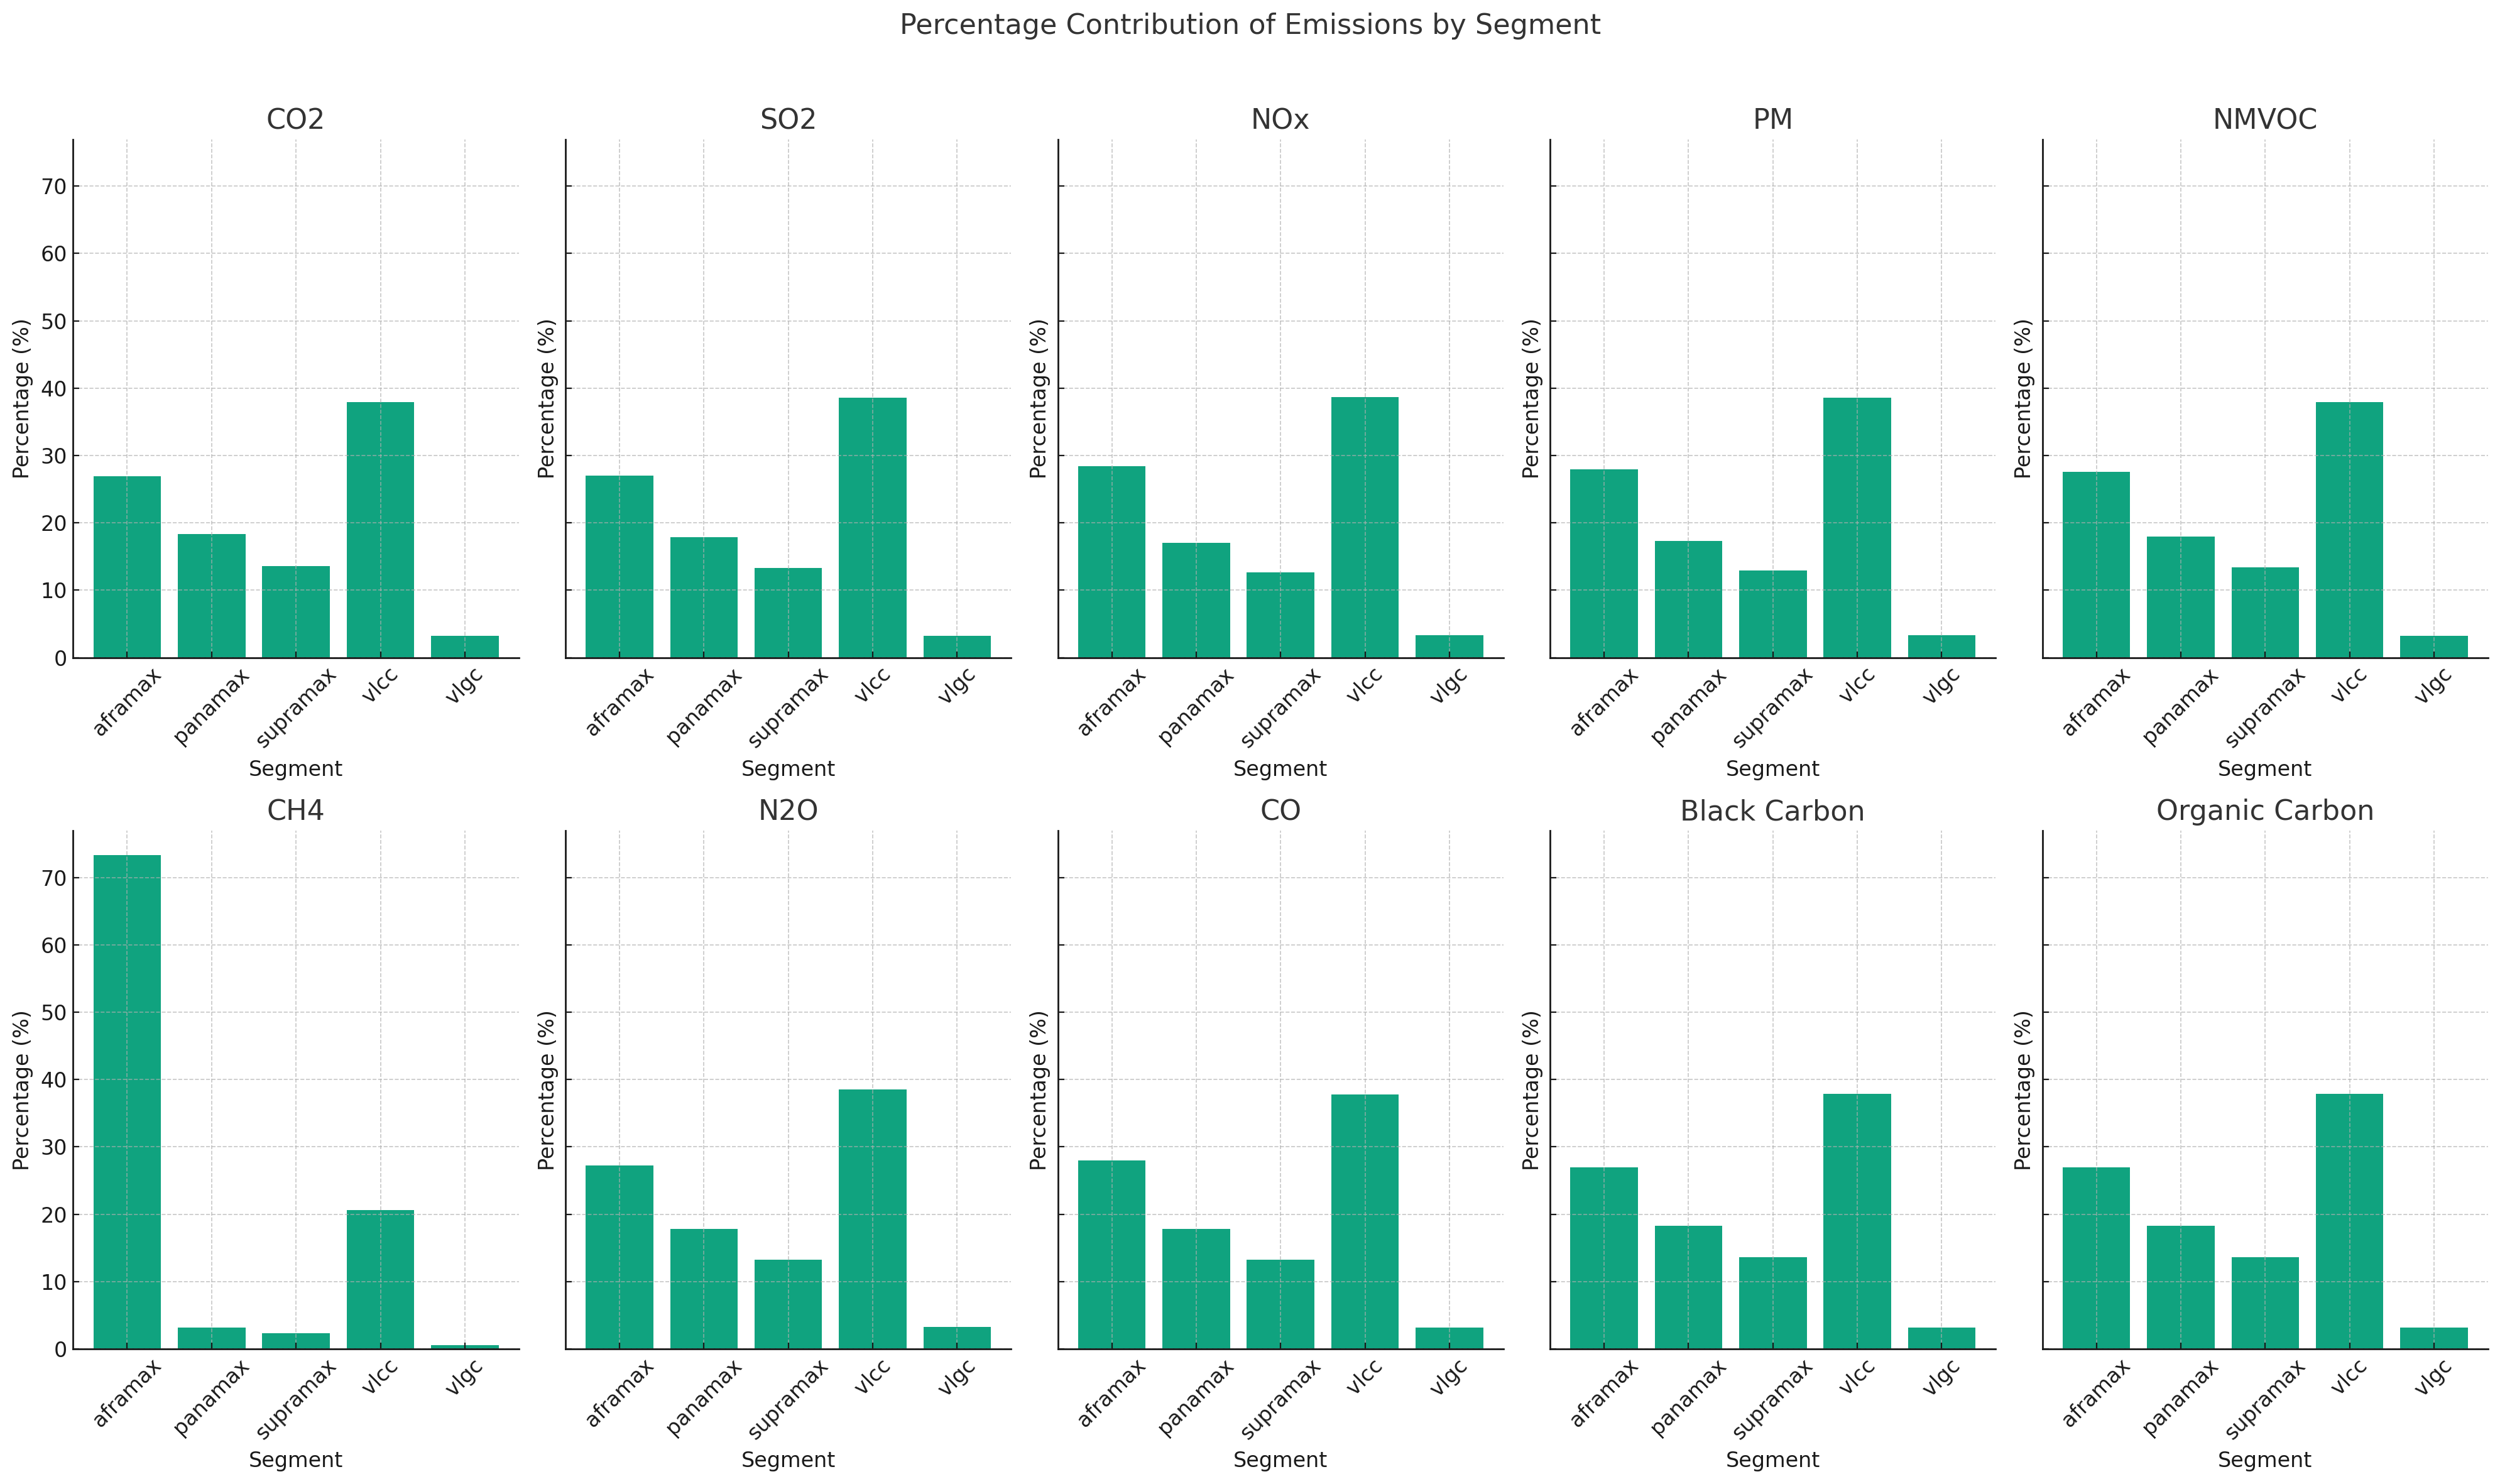
\includegraphics[width=0.8\textwidth]{images/segment_emissions.png}
    \caption{Percentage of Emissions by Segment}
    \label{segment_emissions}
\end{figure}

Figure \ref{segment_emissions} shows percentage of emissions by segment.
The analysis reveals a diverse emission profile across segments such as VLCC, VLG, Aframax, Panamax, Capesize, and Supramax. 
Notably, the VLCC segment emerges as a significant contributor to emissions such as CO2, SO2, and NOx, highlighting potential areas for emission reduction strategies.